\documentclass[tikz,border=3.14mm]{standalone}
\usetikzlibrary{3d}

\colorlet{green_set}{green!70!black}
\colorlet{purple_set}{blue!80!cyan!60!red!95!black!90}
\colorlet{red_set}{red!80!black}
\colorlet{orange_set}{orange!80!}

\begin{document}
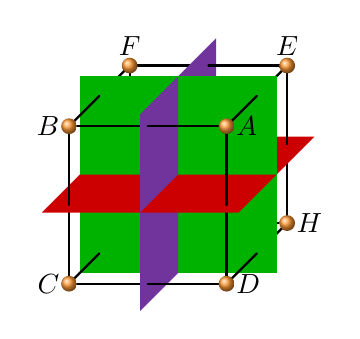
\begin{tikzpicture}[line cap=round,line join=round]

\def\axisX{(1cm,0cm)}
\def\axisY{(0cm,1cm)}
\def\axisZ{(0.35cm,0.35cm)}

% Define the points as coordinates
\coordinate (A) at (1,1,1);
\coordinate (B) at (-1,1,1);
\coordinate (C) at (-1,-1,1);
\coordinate (D) at (1,-1,1);
\coordinate (E) at (1,1,-1);
\coordinate (F) at (-1,1,-1);
\coordinate (G) at (-1,-1,-1);
\coordinate (H) at (1,-1,-1);

%-----------------------------------------------
%-----------------------------------------------
\draw[line width=0.8pt] (G) -- (-1,0,-1);
\fill[red_set,opacity=1.0] (-1.25,0,-1.25) -- (-1.25,0,0) -- (0,0,0) -- (0,0,-1.25) -- cycle;
\draw[line width=0.8pt] (F) -- (-1,0,-1);

\draw[line width=0.8pt] (0,-1,1) -- (C);

\draw[line width=0.8pt] (0,-1,-1) -- (G);

\draw[line width=0.8pt] (0,1,-1) -- (F);
\fill[purple_set,opacity=1.0] (0,-1.25,-1.25) -- (0,-1.25,0) -- (0,1.25,0) -- (0,1.25,-1.25) -- cycle;

\draw[line width=0.8pt] (H) -- (0,-1,-1);
\draw[line width=0.8pt] (E) -- (0,1,-1);

%-----------------------------------------------
\draw[line width=0.8pt] (H) -- (1,0,-1);
\fill[red_set,opacity=1.0] (1.25,0,-1.25) -- (1.25,0,0) -- (0,0,0) -- (0,0,-1.25) -- cycle;
%-----------------------------------------------

\draw[line width=0.8pt] (1,1,0) -- (E);

\draw[line width=0.8pt] (-1,1,0) -- (F);

\draw[line width=0.8pt] (-1,-1,0) -- (G);
\shade[shading=ball, ball color=orange_set] (G) circle (.1cm);

\draw[line width=0.8pt] (1,-1,0) -- (H);

% (-,-,here) plane
\fill[green_set,opacity=1.0] (1.25,1.25,0) -- (-1.25,1.25,0) -- (-1.25,-1.25,0) -- (1.25,-1.25,0) -- cycle;

\draw[line width=0.8pt] (A) -- (1,1,0);
\draw[line width=0.8pt] (B) -- (-1,1,0);
\draw[line width=0.8pt] (C) -- (-1,-1,0);
\draw[line width=0.8pt] (D) -- (1,-1,0);

%-----------------------------------------------
%-----------------------------------------------
\draw[line width=0.8pt]  (C) -- (-1,0,1);
\fill[red_set,opacity=1.0] (-1.25,0,1.25) -- (-1.25,0,0) -- (0,0,0) -- (0,0,1.25) -- cycle;

\draw[line width=0.8pt] (0,1,1) -- (B);
% (here,-,-) plane
\fill[purple_set,opacity=1.0] (0,1.25,1.25) -- (0,1.25,0) -- (0,-1.25,0) -- (0,-1.25,1.25) -- cycle;

\draw[line width=0.8pt] (A) -- (0,1,1);
\draw[line width=0.8pt] (D) -- (0,-1,1);

%-----------------------------------------------
%-----------------------------------------------
\draw[line width=0.8pt] (D) -- (1,0,1);

\fill[red_set,opacity=1.0] (1.25,0,1.25) -- (1.25,0,0) -- (0,0,0) -- (0,0,1.25) -- cycle;

\draw[line width=0.8pt] (A) -- (1,0,1);
\draw[line width=0.8pt]  (B) -- (-1,0,1);
\draw[line width=0.8pt] (E) -- (1,0,-1);
%-----------------------------------------------
% Draw balls at the corners of the cube
\shade[shading=ball, ball color=orange_set] (A) circle (.1cm);
\shade[shading=ball, ball color=orange_set] (B) circle (.1cm);
\shade[shading=ball, ball color=orange_set] (C) circle (.1cm);
\shade[shading=ball, ball color=orange_set] (D) circle (.1cm);
\shade[shading=ball, ball color=orange_set] (E) circle (.1cm);
\shade[shading=ball, ball color=orange_set] (F) circle (.1cm);
\shade[shading=ball, ball color=orange_set] (H) circle (.1cm);
%-----------------------------------------------

% Label the points
\foreach \point/\position in {A/right,B/left,C/left,D/right,E/above,F/above,H/right}
{
  \node[\position] at (\point) {$\point$};
}

\end{tikzpicture}
\end{document}